\subsection{Analytisches Haar-Wavelet}
\rhead{Analytisches Haar-Wavelet}
Betrachten wir zum Abschluss noch beispielhaft das Haar-Wavelet.
In diesem Abschnitt sei es zentriert um $t=0$.
Diese symmetrie wird sich im Folgenden als hilfreich erweisen.
\[
	\psi_{\text{Haar}} = \left\lbrace\begin{matrix*}[r]
		1 & -\frac{1}{2} \le t < 0  \\
		-1 & 0 \le t < \frac{1}{2} \\
		0 & \text{sonst}
	\end{matrix*} \right..
\]
Die Hilbert-Transformierte des Haar-Wavelets berechnet sich zu
\begin{align*}
	\mathcal{H} \psi_{\text{Haar}}
	&= \frac{1}{\pi} \int_{-\infty}^{\infty} \frac{\psi_{\text{Haar}}(x)}{t-x} dx\\
	&= \frac{1}{\pi}\left( \int_{-0.5}^{0} \frac{1}{t-x}dx + \int_{0}^{0.5} \frac{-1}{t-x}dx \right)\\
	&= \frac{1}{\pi} \left( -\left[\log \left|t-x\right| \right]_{-0.5}^{0} + \left[\log\left|t-x\right| \right]_{0}^{0.5} \right)\\
	&= \frac{1}{\pi} \left( -\log\left|t\right| + \log\left|t+0.5\right| + \log\left|t-0.5\right| - \log\left|t\right|\right)\\
	&= \frac{1}{\pi} \log\left|\frac{(t+0.5)(t-0.5)}{t^2}\right|
	= \frac{1}{\pi} \log\left|\frac{t^2-0.5^2}{t^2}\right|.
\end{align*}
Die analytische Form des Haar-Wavelet ist nach Gelcihung~\eqref{complex:anawave} also
\[
 \psi^\ast_{\text{Haar}} = \frac{1}{\sqrt{2}}\left(\psi_{\text{Haar}} + \frac{i}{\pi} \log\left|\frac{t^2-0.5^2)}{t^2}\right|\right).
\]
Diese Funktion ist in Abbildung~\ref{complex:haar} dargestellt.
Das analytische Haar-Wavelet hat offensichtlich keinen kompakten Träger mehr.
Gut ersichtlich ist jedoch die Symmetrie.
Der Realteil ist eine ungerade Funktion, folglich ist der Imaginärteil gerade.
Die graue Fläche zeigt den Betrag der Funktion.
Bei analytischen Wavelets ist der Betrag gleich der Envelope.
Die Energie des analysierten Signals geht also immer entweder in den Real- oder den Imaginärteil der Analyse, was sich wieder in der gewünschten Eigenschaft zeigt, Amplitude und Phase unabhängig betrachten zu können.

\begin{figure}
	\centering
	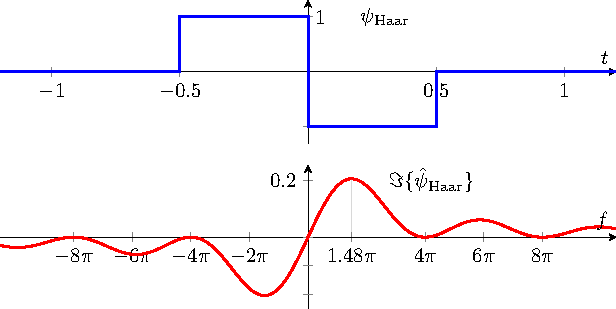
\includegraphics{papers/complex/images/haar.pdf}
	\caption{Das analytische Haar-Wavelet, Realteil in Blau und Imaginärteil in Rot. \label{complex:haar}}
\end{figure}